\section{Theorie}
\label{sec:Theorie}
Das Ziel dieses Versuchs ist es, die Suszeptibilität $\chi$ paramanetischer Substanzen zu bestimmen.
Der Diamagnetismus hängt mit dem Atomaren Drehimpuls zusammen, dieser darf bei einem Paramagneten nicht verschwinden. 
Da Ionen seltener Erden Elektronen besitzen die einen großen Bahndrehimpuls haben und somit einen großen nicht verschwindenden 
Drehimpuls, nutzen wir in diesem Fall besagte Ionen seltener Erden.

\paragraph{Theoretische Bestimmung von $\chi$}
Im Vakuum gilt für die magnetische Flussdichte $\vec{B}$ und die magnetische Feldstärke $\vec{H}$ der Zusammenhang 
\begin{equation}
    \label{equ:1}
    \vec{B} = \mu_0 \vec{H},
\end{equation}
mit der Induktionskonstanten $\mu_0$.
Für die Magnetisierung $\vec{M}$ gilt mit \eqref{equ:1}
\begin{equation}
    \label{equ:2}
    \vec{M} = \mu_0 \chi \vec{H}.
\end{equation}
Dabei ist $\chi$ keine Konstante, sondern hängt von $H$ und der Temperatur T ab.
Um diese Temperaturabhängigkeit zu bestimmen, wird das mittlere magnetische Moment $\bar{\mu}$ in Gleichung \eqref{equ:3},
mit hilfe des Bohrschen Magneton $\mu_B$, dem Landre-Faktor $g_J$ \eqref{equ:7}, der Boltzmann-Konstante $k$ und der Geamtdrehimpulsquantenzahl $J$,
beschrieben,
\begin{equation}
    \label{equ:3}
    \bar{\mu} = - \mu_B g_J \frac{\sum_{m = -J}^{J}\, m\, \text{exp}\left( \frac{-\mu_B g_J mB}{k T}\right)} {\sum_{m = -J}^{J}\, \text{exp}\left( \frac{-\mu_B g_J mB}{k T}\right)},
\end{equation}
woraus für $M$ die Brillouin-Funktion \eqref{equ:4} folgt.
\begin{equation}
    \label{equ:4}
    M = \mu_0 N \bar{\mu}.
\end{equation}
Der komplexe Zusammenhang in Gleichung \eqref{equ:3} lässt sich für Zimmertemperaturen und Magnetfeldern der Größenordnung 1 Tesla 
näherungsweise vereinfachen, woraus sich für $M$ 
\begin{equation}
    \label{equ:5}
    M = \frac{1}{3} \mu_0 \mu_B^2 g_J^2 N \frac{J(J + 1) B}{k T},
\end{equation}
ergibt und mit Hilfe von Gleichung \eqref{equ:1} und \eqref{equ:2} die paramagnetische Suszibilität durch Gleichung \eqref{equ:6} bestimmt werden kann.
\begin{equation}
    \label{equ:6}
    \chi = \frac{\mu_0 \mu_B^2 g_J^2 N J (J + 1)}{3 k T}.
\end{equation}
Der Landre-Faktor ist gegeben durch 
\begin{equation}
    \label{equ:7}
    g_J := \frac{3 J(J + 1) + {S(S+1) - L(L+1)}}{2 J(J+1)},
\end{equation}
mit $S$ der Spinquantenzahl des Atoms und  $L$ dem Bahndrehimpuls des Atoms.

\paragraph{Praktische Bestimmung von $\chi$}
Für die praktische Messung von $\chi$ werden zwei möglichst gleiche Spulen wie in Abbildung \ref{fig:1}, als Brückenschaltung 
geschaltet. Dabei kann die Spule mit der Induktivität $L_M$, mit der Probe gefüllt werden. $R$ und $R_M$ stellen dabei die Verlustwiederstände der 
beiden Spulen dar.
\begin{figure}
    \centering
    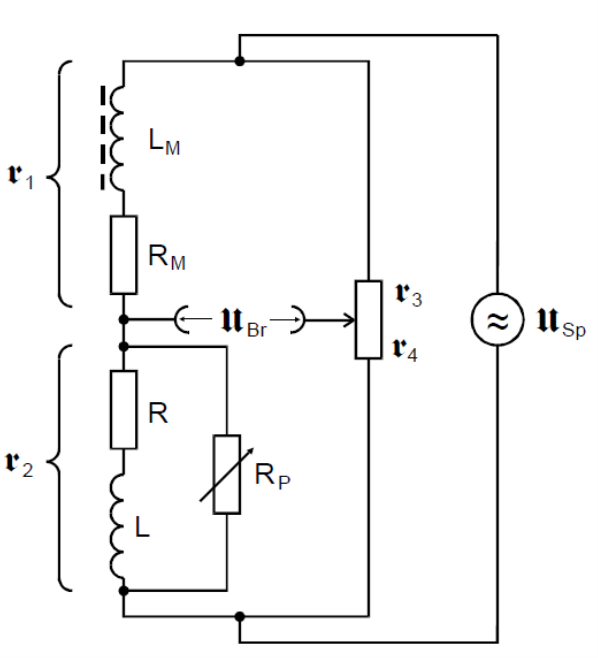
\includegraphics[width = 0.50\textwidth]{V606Bild1.png}
    \caption{Schematische Brückenschaltung.}
    \label{fig:1}
\end{figure}
Für die erste Methode zur Bestimmung von $\chi$, wird die Brückenspannung abgeglichen, das heißt die Brückenspannung $U_{Br}$ wird durch Variation von $R_3$ möglichst gering gewählt.
Anschließend wird die Probe in die Spule geschoben und die Brückenspannung gemessen.
Die Suszibilität der Probe in der Spule, lässt sich nun für hohe Messfrequenzen berechnen.
\begin{equation}
    \label{equ:8}
    \chi = 4 \frac{F}{Q} \frac{U_{Br}}{U_{Sp}}.
\end{equation}
Dabei sind $U_{Sp}$ die Brückenspannung, F der Querschnitt der Spule und Q der Querschnitt der Probe.

Bei der zweiten Methode wird wieder erst die Brückenspannung abgeglichen und dann die Probe eingefügt. Danach wird jedoch nicht $U_{Br}$ gemessen, 
sondern die Brückenspannung mit enthaltener Probe abgeglichen, als versuch diese möglichst gering zu halten. 
Aus der Variation des Widerstandes $R_3$ beim Abgleichen ohne und mit Probe $\increment R$ lässt sich nun ebenfalls $\chi$ berechnen.
\begin{equation}
    \label{equ:9}
    \chi = 2 \frac{\increment R }{R_3} \frac{F}{Q}.
\end{equation}
Dabei ist $R_3$ der Widerstand $R_3$ nach Abgleich der Brückenspannung ohne Probe.

\paragraph{Selektivverstärker}
Da die gemessene Brückenspannung sehr klein ist und somit in der selben Größenordnung wie die Störspannung an den Ausgangsklemmen der Brückenschaltung ist, 
wird ein Selektivverstärker genutzt. Dieser Selektivverstärker lässt vorrangig eine bestimmte Frequenz bzw. einen  gewissen Frequenzbereich pssieren.
Da die Signalspannung monofrequent ist, Wird der Selektivverstärker so eingestellt, dass eben diese Signalfrequenz durchgelassen wird, wodurch ein großteil der 
Störspannung abgeschirmt wird. Zudem verstäkt er das Signal um das zehnfache, um genauere Messungen durchführen zu können. 
Als Maß der Wirksamkeit des Selektivverstärkers gilt die Breite der in Abbildung \ref{fig:2} dargestellten Filterkurve oder auch die güte G
\begin{equation}
    \label{equ:10}
    O = \frac{v_0}{v_+ - v_-}.
\end{equation}
$v_0$ ist die eigentlich gewünschte Durchlassfrequenz und sollte die Frequenz sein, bei der der Quotient der Ausgangsspannung $U_A$ und der Eingangsspannung $U_E$ 
eins ist bzw. sein Maximum erreicht. $v_-$ und $v_+$ sind die Frequenzen, bei denen wie in Abbildung \ref{fig:2} dargestellt, der Quotient $\frac{U_A}{U_E}$ den Wert $\frac{1}{\sqrt{2}}$ besitzt.
\begin{figure}
    \centering
    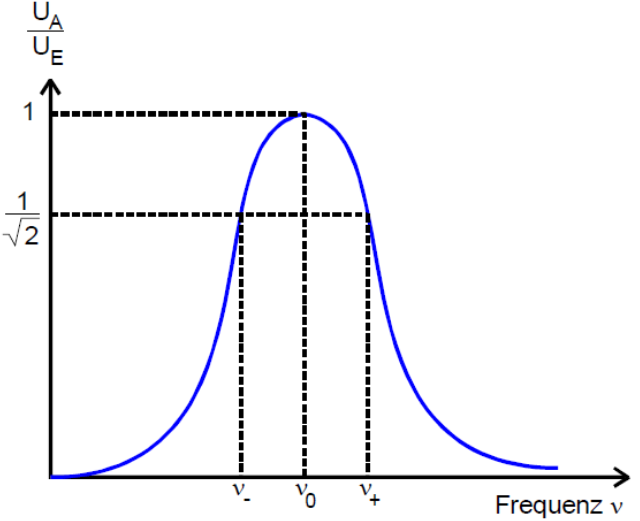
\includegraphics[width = 0.60\textwidth]{V606Bild2.png}
    \caption{Filterkurve eines Selektivverstärkers.}
    \label{fig:2}
\end{figure}

